\documentclass[tikz, border=12pt]{standalone}
\usepackage{tikz}
\usepackage{amsmath}
\usetikzlibrary{arrows.meta, shapes.geometric, positioning, fit, backgrounds, calc}

\begin{document}
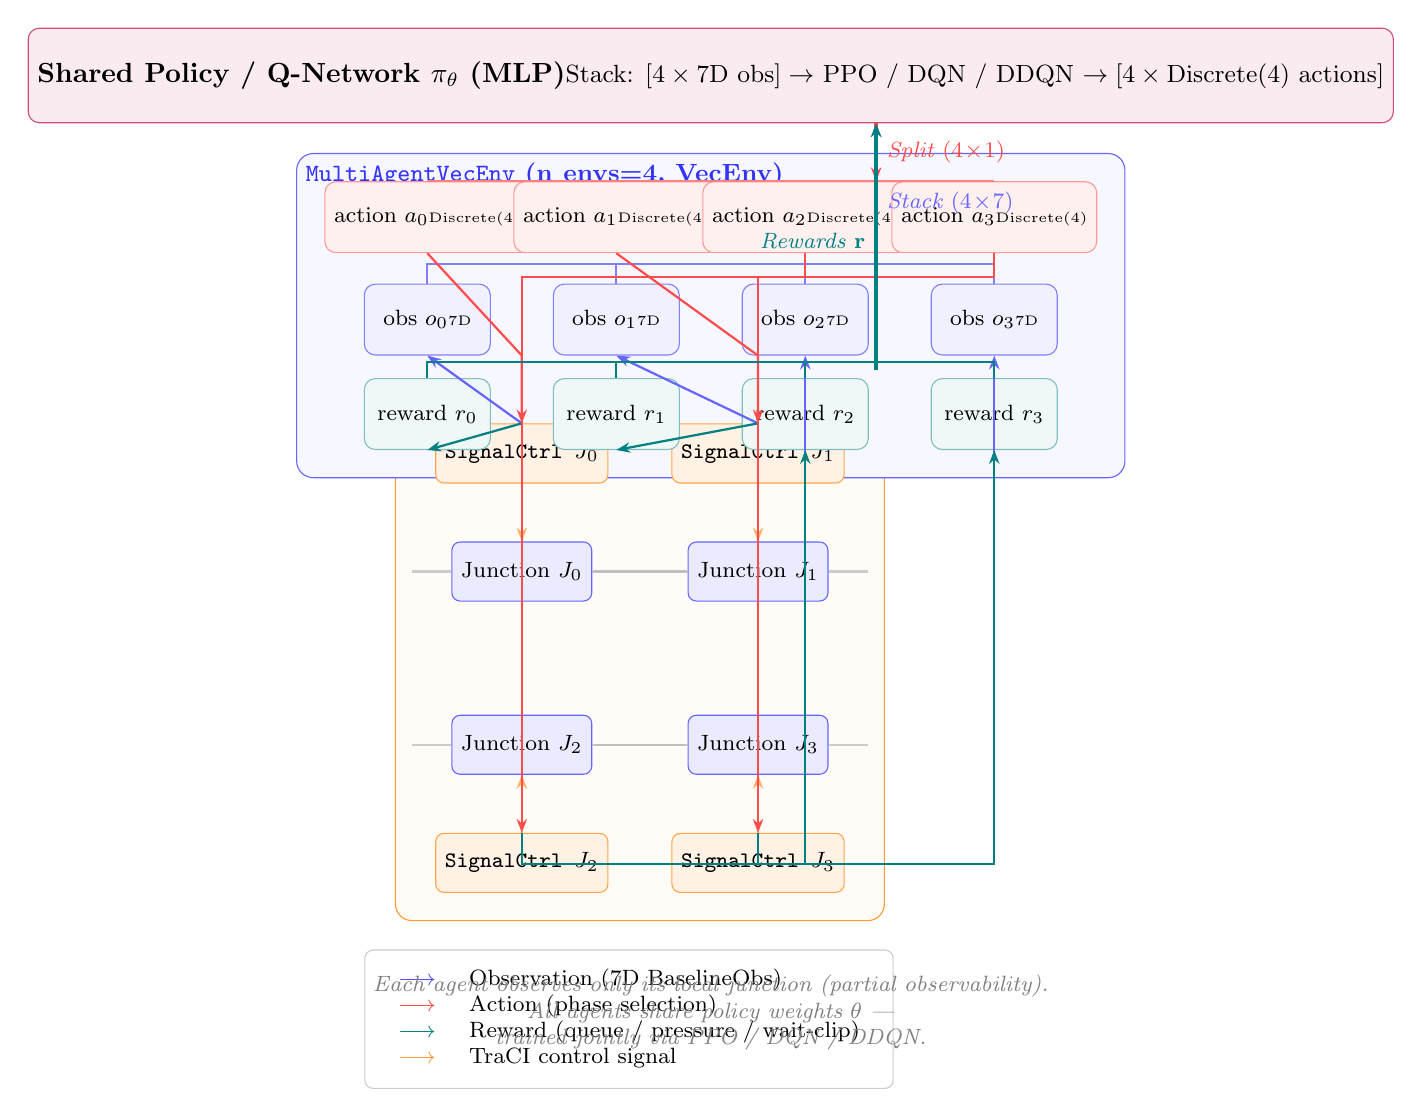
\begin{tikzpicture}[
    box/.style={
        rectangle, draw, rounded corners=4pt,
        text centered, font=\small, fill=white,
        minimum height=0.9cm
    },
    jbox/.style={
        rectangle, draw=blue!60, rounded corners=3pt,
        text centered, font=\footnotesize,
        fill=blue!8, minimum width=2.0cm, minimum height=0.75cm
    },
    sbox/.style={
        rectangle, draw=orange!70, rounded corners=3pt,
        text centered, font=\footnotesize,
        fill=orange!10, minimum width=2.0cm, minimum height=0.75cm
    },
    bigframe/.style={
        rectangle, draw, rounded corners=6pt,
        font=\small\bfseries, fill=gray!6, inner sep=10pt
    },
    arrow/.style={-{Stealth[length=5pt]}, thick},
    darrow/.style={-{Stealth[length=5pt]}, thick, dashed, gray},
    redarrow/.style={-{Stealth[length=5pt]}, thick, red!70},
    bluearrow/.style={-{Stealth[length=5pt]}, thick, blue!60},
    greenarrow/.style={-{Stealth[length=5pt]}, thick, teal},
]

%% ═══════════════════════════════════════════════════════
%% LAYER 1 — SUMO SIMULATION (bottom)
%% ═══════════════════════════════════════════════════════

% 2x2 grid junctions
\node[jbox, minimum width=1.6cm] (J00) at (0, 0)    {Junction $J_0$};
\node[jbox, minimum width=1.6cm] (J10) at (3, 0)    {Junction $J_1$};
\node[jbox, minimum width=1.6cm] (J01) at (0,-2.2)  {Junction $J_2$};
\node[jbox, minimum width=1.6cm] (J11) at (3,-2.2)  {Junction $J_3$};

% Roads between junctions
\draw[thick, gray!50] (J00.east)  -- (J10.west);
\draw[thick, gray!50] (J01.east)  -- (J11.west);
\draw[thick, gray!50] (J00.south) -- (J01.north);
\draw[thick, gray!50] (J10.south) -- (J11.north);

% External roads
\draw[thick, gray!40] (J00.north)  -- ++(0, 0.5);
\draw[thick, gray!40] (J10.north)  -- ++(0, 0.5);
\draw[thick, gray!40] (J01.south)  -- ++(0,-0.5);
\draw[thick, gray!40] (J11.south)  -- ++(0,-0.5);
\draw[thick, gray!40] (J00.west)   -- ++(-0.5, 0);
\draw[thick, gray!40] (J01.west)   -- ++(-0.5, 0);
\draw[thick, gray!40] (J10.east)   -- ++(0.5, 0);
\draw[thick, gray!40] (J11.east)   -- ++(0.5, 0);

% SUMO frame
\begin{scope}[on background layer]
  \node[bigframe, draw=orange!60, fill=orange!5,
        fit=(J00)(J10)(J01)(J11),
        label={[anchor=north west, font=\small\bfseries, text=orange!80]
               north west:SUMO Simulation (libsumo)}
       ] (sumoframe) {};
\end{scope}

%% ═══════════════════════════════════════════════════════
%% LAYER 2 — TrafficControlEnv + SignalControllers
%% ═══════════════════════════════════════════════════════

\node[sbox, minimum width=2.1cm] (SC0) at (0,  1.5) {\texttt{SignalCtrl $J_0$}};
\node[sbox, minimum width=2.1cm] (SC1) at (3,  1.5) {\texttt{SignalCtrl $J_1$}};
\node[sbox, minimum width=2.1cm] (SC2) at (0, -3.7) {\texttt{SignalCtrl $J_2$}};
\node[sbox, minimum width=2.1cm] (SC3) at (3, -3.7) {\texttt{SignalCtrl $J_3$}};

% SignalCtrl ↔ Junction (double arrow)
\draw[arrow, orange!60] (SC0.south) -- (J00.north);
\draw[arrow, orange!60] (SC1.south) -- (J10.north);
\draw[arrow, orange!60] (SC2.north) -- (J01.south);
\draw[arrow, orange!60] (SC3.north) -- (J11.south);

% TrafficControlEnv frame
\begin{scope}[on background layer]
  \node[bigframe, draw=orange!80, fill=orange!3,
        fit=(SC0)(SC1)(SC2)(SC3)(sumoframe),
        label={[anchor=north west, font=\small\bfseries, text=orange!90]
               north west:\texttt{TrafficControlEnv} (single\_agent=False)}
       ] (envframe) {};
\end{scope}

%% ═══════════════════════════════════════════════════════
%% LAYER 3 — MultiAgentVecEnv
%% ═══════════════════════════════════════════════════════

% Obs cache boxes
\node[box, fill=blue!6, draw=blue!50, minimum width=1.6cm, font=\footnotesize]
    (obs0) at (-1.2, 3.2) {obs $o_0$\\{\tiny 7D}};
\node[box, fill=blue!6, draw=blue!50, minimum width=1.6cm, font=\footnotesize]
    (obs1) at ( 1.2, 3.2) {obs $o_1$\\{\tiny 7D}};
\node[box, fill=blue!6, draw=blue!50, minimum width=1.6cm, font=\footnotesize]
    (obs2) at ( 3.6, 3.2) {obs $o_2$\\{\tiny 7D}};
\node[box, fill=blue!6, draw=blue!50, minimum width=1.6cm, font=\footnotesize]
    (obs3) at ( 6.0, 3.2) {obs $o_3$\\{\tiny 7D}};

% Action boxes
\node[box, fill=red!6, draw=red!40, minimum width=1.6cm, font=\footnotesize]
    (act0) at (-1.2, 4.5) {action $a_0$\\{\tiny Discrete(4)}};
\node[box, fill=red!6, draw=red!40, minimum width=1.6cm, font=\footnotesize]
    (act1) at ( 1.2, 4.5) {action $a_1$\\{\tiny Discrete(4)}};
\node[box, fill=red!6, draw=red!40, minimum width=1.6cm, font=\footnotesize]
    (act2) at ( 3.6, 4.5) {action $a_2$\\{\tiny Discrete(4)}};
\node[box, fill=red!6, draw=red!40, minimum width=1.6cm, font=\footnotesize]
    (act3) at ( 6.0, 4.5) {action $a_3$\\{\tiny Discrete(4)}};

% Reward boxes
\node[box, fill=teal!6, draw=teal!50, minimum width=1.6cm, font=\footnotesize]
    (rew0) at (-1.2, 2.0) {reward $r_0$};
\node[box, fill=teal!6, draw=teal!50, minimum width=1.6cm, font=\footnotesize]
    (rew1) at ( 1.2, 2.0) {reward $r_1$};
\node[box, fill=teal!6, draw=teal!50, minimum width=1.6cm, font=\footnotesize]
    (rew2) at ( 3.6, 2.0) {reward $r_2$};
\node[box, fill=teal!6, draw=teal!50, minimum width=1.6cm, font=\footnotesize]
    (rew3) at ( 6.0, 2.0) {reward $r_3$};

% arrows SC → obs, SC → rew
\draw[bluearrow] (SC0.north) -- (obs0.south);
\draw[bluearrow] (SC1.north) -- (obs1.south);
\draw[bluearrow] (SC2.north) -- ++(0,-0.4) -| (obs2.south);  % reroute SC2
\draw[bluearrow] (SC3.north) -- ++(0,-0.4) -| (obs3.south);  % reroute SC3

\draw[greenarrow] (SC0.north) -- (rew0.south);
\draw[greenarrow] (SC1.north) -- (rew1.south);
\draw[greenarrow] (SC2.north) -- ++(0,-0.4) -| (rew2.south);
\draw[greenarrow] (SC3.north) -- ++(0,-0.4) -| (rew3.south);

% MultiAgentVecEnv frame
\begin{scope}[on background layer]
  \node[bigframe, draw=blue!60, fill=blue!3,
        fit=(obs0)(obs1)(obs2)(obs3)(act0)(act1)(act2)(act3)(rew0)(rew1)(rew2)(rew3),
        label={[anchor=north west, font=\small\bfseries, text=blue!80]
               north west:\texttt{MultiAgentVecEnv} (n\_envs=4, VecEnv)}
       ] (vecframe) {};
\end{scope}

%% ═══════════════════════════════════════════════════════
%% LAYER 4 — Shared Policy / Q-Network
%% ═══════════════════════════════════════════════════════

\node[box, draw=purple!70, fill=purple!8,
      minimum width=8cm, minimum height=1.2cm,
      font=\normalsize] (policy) at (2.4, 6.3) {
    \textbf{Shared Policy / Q-Network $\pi_\theta$ (MLP)}\\
    {\small Stack: $[4 \times 7\text{D obs}] \rightarrow$ PPO / DQN / DDQN $\rightarrow [4 \times \text{Discrete}(4)\text{ actions}]$}
};

% obs stacking arrow
\draw[bluearrow, line width=1.2pt]
    ($(obs0.north)!0.5!(obs3.north) + (2.1,0)$) coordinate (midobs)
    -- node[right, font=\footnotesize\it]{Stack $(4\!\times\!7)$}
    (policy.south -| midobs);

% draw a bracket-like collector from obs boxes to midobs
\draw[blue!50, thick] (obs0.north) -- ++(0,0.25) -| (midobs);
\draw[blue!50, thick] (obs1.north) -- ++(0,0.25) -| (midobs);
\draw[blue!50, thick] (obs2.north) -- ++(0,0.25) -| (midobs);
\draw[blue!50, thick] (obs3.north) -- ++(0,0.25) -| (midobs);

% policy → actions
\coordinate (midact) at ($(act0.north)!0.5!(act3.north) + (2.1,0)$);
\draw[redarrow, line width=1.2pt]
    (policy.south -| midact)
    -- node[right, font=\footnotesize\it]{Split $(4\!\times\!1)$}
    (midact);
\draw[red!50, thick] (midact) |- (act0.north);
\draw[red!50, thick] (midact) |- (act1.north);
\draw[red!50, thick] (midact) |- (act2.north);
\draw[red!50, thick] (midact) |- (act3.north);

% actions → SignalCtrl (down)
\draw[redarrow] (act0.south) -- (SC0.north |- obs0.south) -- (SC0.north);
\draw[redarrow] (act1.south) -- (SC1.north |- obs1.south) -- (SC1.north);
\draw[redarrow] (act2.south) -- ++(0,-0.3) -| (SC2.north);
\draw[redarrow] (act3.south) -- ++(0,-0.3) -| (SC3.north);

% reward collector → policy (for update)
\coordinate (midrew) at ($(rew0.north)!0.5!(rew3.north) + (2.1,0.1)$);
\draw[teal, thick] (rew0.north) -- ++(0,0.2) -| (midrew);
\draw[teal, thick] (rew1.north) -- ++(0,0.2) -| (midrew);
\draw[teal, thick] (rew2.north) -- ++(0,0.2) -| (midrew);
\draw[teal, thick] (rew3.north) -- ++(0,0.2) -| (midrew);
\draw[greenarrow, line width=1.2pt]
    (midrew) -- ++(0, 0.15)
    -- node[left, font=\footnotesize\it, text=teal]{Rewards $\mathbf{r}$}
    (policy.south -| midrew);

%% ═══════════════════════════════════════════════════════
%% LEGEND
%% ═══════════════════════════════════════════════════════
\node[anchor=north west, draw=gray!40, rounded corners=3pt, fill=white,
      inner sep=6pt, font=\footnotesize] at (-2.0, -4.8) {
    \begin{tabular}{ll}
        \textcolor{blue!70}{$\longrightarrow$} & Observation (7D BaselineObs) \\
        \textcolor{red!70}{$\longrightarrow$}  & Action (phase selection) \\
        \textcolor{teal}{$\longrightarrow$}    & Reward (queue / pressure / wait-clip) \\
        \textcolor{orange!80}{$\longrightarrow$} & TraCI control signal \\
    \end{tabular}
};

%% ═══════════════════════════════════════════════════════
%% CAPTION NOTE
%% ═══════════════════════════════════════════════════════
\node[font=\footnotesize\it, text=gray, text width=10cm, align=center]
    at (2.4, -5.6) {
    Each agent observes only its local junction (partial observability).\\
    All agents share policy weights $\theta$ — trained jointly via PPO / DQN / DDQN.
};

\end{tikzpicture}
\end{document}
